\section{Chapter Two: Data Analysis and Visualization}

\subsection{Visual Representation}
Here is a picture we included to demonstrate image handling.

\begin{figure}[h]
    \centering
    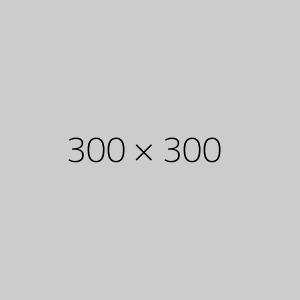
\includegraphics[width=0.5\textwidth]{photo.jpeg}
    \caption{A sample image included in the document. If missing, a placeholder should appear.}
\end{figure}

\subsection{Tabular Data}
We present complex data in the following tables.

\begin{table}[h]
    \centering
    \begin{tabular}{llr}
        \toprule
        \multicolumn{2}{c}{Item} \\
        \cmidrule(r){1-2}
        Animal & Description & Price (\$) \\
        \midrule
        Gnat  & per gram & 13.65 \\
        & each     & 0.01 \\
        Gnu   & stuffed  & 92.50 \\
        Emu   & stuffed  & 33.33 \\
        Armadillo & frozen & 8.99 \\
        \bottomrule
    \end{tabular}
    \caption{A sample table using booktabs.}
\end{table}

\lipsum[51-55]

\subsection{Long Table Example}
For larger datasets that span multiple pages, we use the longtable environment.

\begin{longtable}{p{0.3\textwidth} p{0.6\textwidth}}
    \caption{A Long Table Example}\\
    \toprule
    \textbf{Concept} & \textbf{Definition} \\
    \midrule
    \endfirsthead
    \toprule
    \textbf{Concept} & \textbf{Definition} \\
    \midrule
    \endhead
    \bottomrule
    \endfoot
    
    Artificial Intelligence & \lipsum[56] \\
    Machine Learning & \lipsum[57] \\
    Deep Learning & \lipsum[58] \\
    Neural Networks & \lipsum[59] \\
    Natural Language Processing & \lipsum[60] \\
    Computer Vision & \lipsum[61] \\
    Robotics & \lipsum[62] \\
\end{longtable}

\subsection{Final Thoughts}
\lipsum[63-75]